\section{Résultats obtenus et perspectives}

\begin{frame}
	\frametitle{Résultats obtenus et perspectives}
	\framesubtitle{Analyse de la fitness}
	\begin{figure}[h]
		\centering
		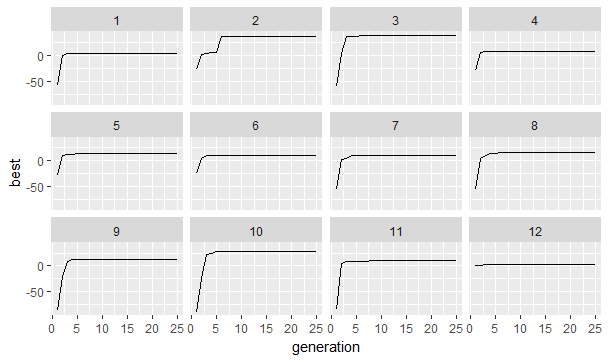
\includegraphics[width=0.9\linewidth]{images/fitness_1_evol}
		\caption{Analyse R pour 1 IA évolutionnaire}
	\end{figure}
\end{frame}

\begin{frame}
	\frametitle{Résultats obtenus et perspectives}
	\framesubtitle{Analyse de la fitness}
	\begin{figure}[h]
		\centering
		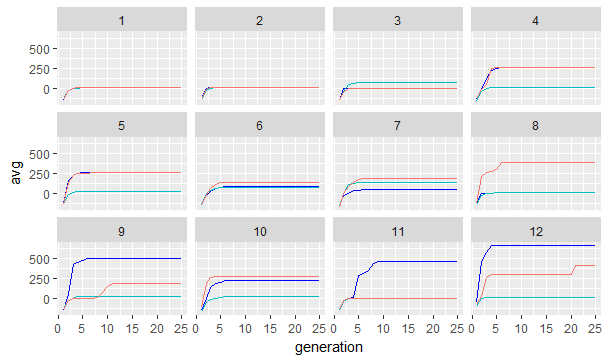
\includegraphics[width=0.9\linewidth]{images/fitness_3_evol}
		\caption{Analyse R pour 3 IA évolutionnaire}
	\end{figure}
\end{frame}

\begin{frame}
	\frametitle{Résultats obtenus et perspectives}
	\framesubtitle{Prévision du tour suivant}
	Exemple de prévision
	\begin{table}
		\centering
		\tiny
		\begin{tabular}{l|c|c|c|c|c|c}
				   & Action 1 & Action 2 & Action 3 & Action 4 & Action 5 & Action 6 \\
			\hline
			Tour 1 & terre & glace & pierre & transaction & pierre & transaction \\
			Prévision 2 & transaction & pierre & transaction & -- & -- & -- \\
			Tour 2 & terre & pierre & transaction & troc & délégation & pierre \\
			Prévision 3 & terre & pierre & transaction & -- & -- & -- \\
			Tour 3 & terre & pierre & transaction & terre & pierre & pierre \\
			Prévision 4 & terre & transaction & pierre & -- & -- & -- \\
			Tour 4 & glace & pierre & terre & glace & terre & transaction \\
		\end{tabular}
	\end{table}
\end{frame}

\begin{frame}
	\frametitle{Résultats obtenus et perspectives}
	\framesubtitle{Analyse des scores}
	\begin{figure}
		\begin{subfigure}{0.4\textwidth}
			\centering
			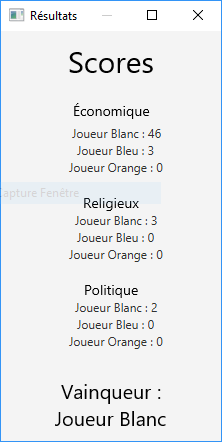
\includegraphics[width=0.5\linewidth]{images/score_evol_vs_random}
			\caption{1 IA évolutionnaire}
		\end{subfigure}
		\begin{subfigure}{0.5\textwidth}
			\centering
			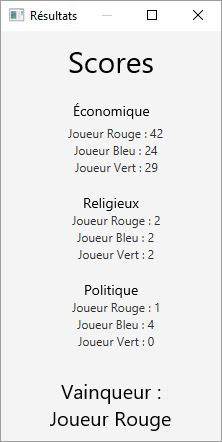
\includegraphics[width=0.4\linewidth]{images/resultats}
			\caption{3 IA évolutionnaire}
		\end{subfigure}
	\end{figure}
\end{frame}